\chapter{Visual scene context recognition through multimodal guidance}

In this chapter, we consider the task of recognizing visual scene context in media content by leveraging pre-trained multimodal information.  
\section{Role of scene as contextual signal}
Visual scene context refers to the global context in the image, including the relationship of the target objects with the environment/location and other co-occurring objects \cite{Bar2004VisualOI}, \cite{Qiao2021ObjectLevelSC}. Visual scene context drives the likelihood of finding particular objects spatially co-located with each other. For example, as shown in Fig \ref{station_kitchen}, utensils are more likely to be present in the kitchen as compared to the train station. 
Apart from the domain of natural scenes, understanding the visual scene context is also important in the case of media content \cite{CMI} esp. movies and curated short content like advertisements. 
\par
In cinematic terms, \textit{mis-en-scene} \cite{Bordwell1979FilmAA} refers to how the different elements of a film are depicted and arranged in front of camera. Key components of \textit{mis-en-scene} include the actors with their different styles, \textbf{visual scenes} where the interactions take place, set design including lighting and camera placement, and the accompanying costumes and makeup of the artists. The visual scene is considered a crucial component since it sets the mood and provides a background for the various actions performed by the actors in the scene. Visual scenes in movies are often tied to social settings like weddings, birthday parties, and workplace gatherings that provide information about character interactions. Accurate recognition of visual scenes can help in uncovering the bias involved in the portrayal of under-represented characters vis-a-vis different scenes, e.g., fewer women shown in the office as compared to the kitchen. For content tagging tasks like genre classification, visual scenes provide context information like battlefield portrayals in action/adventure movies, space-shuttle in sci-fi movies, or courtrooms in dramas.
\par 
In the following section, we highlight certain challenges associated with visual scene recognition, especially w.r.t. movies.
\begin{figure}[h!]
    \centering 
     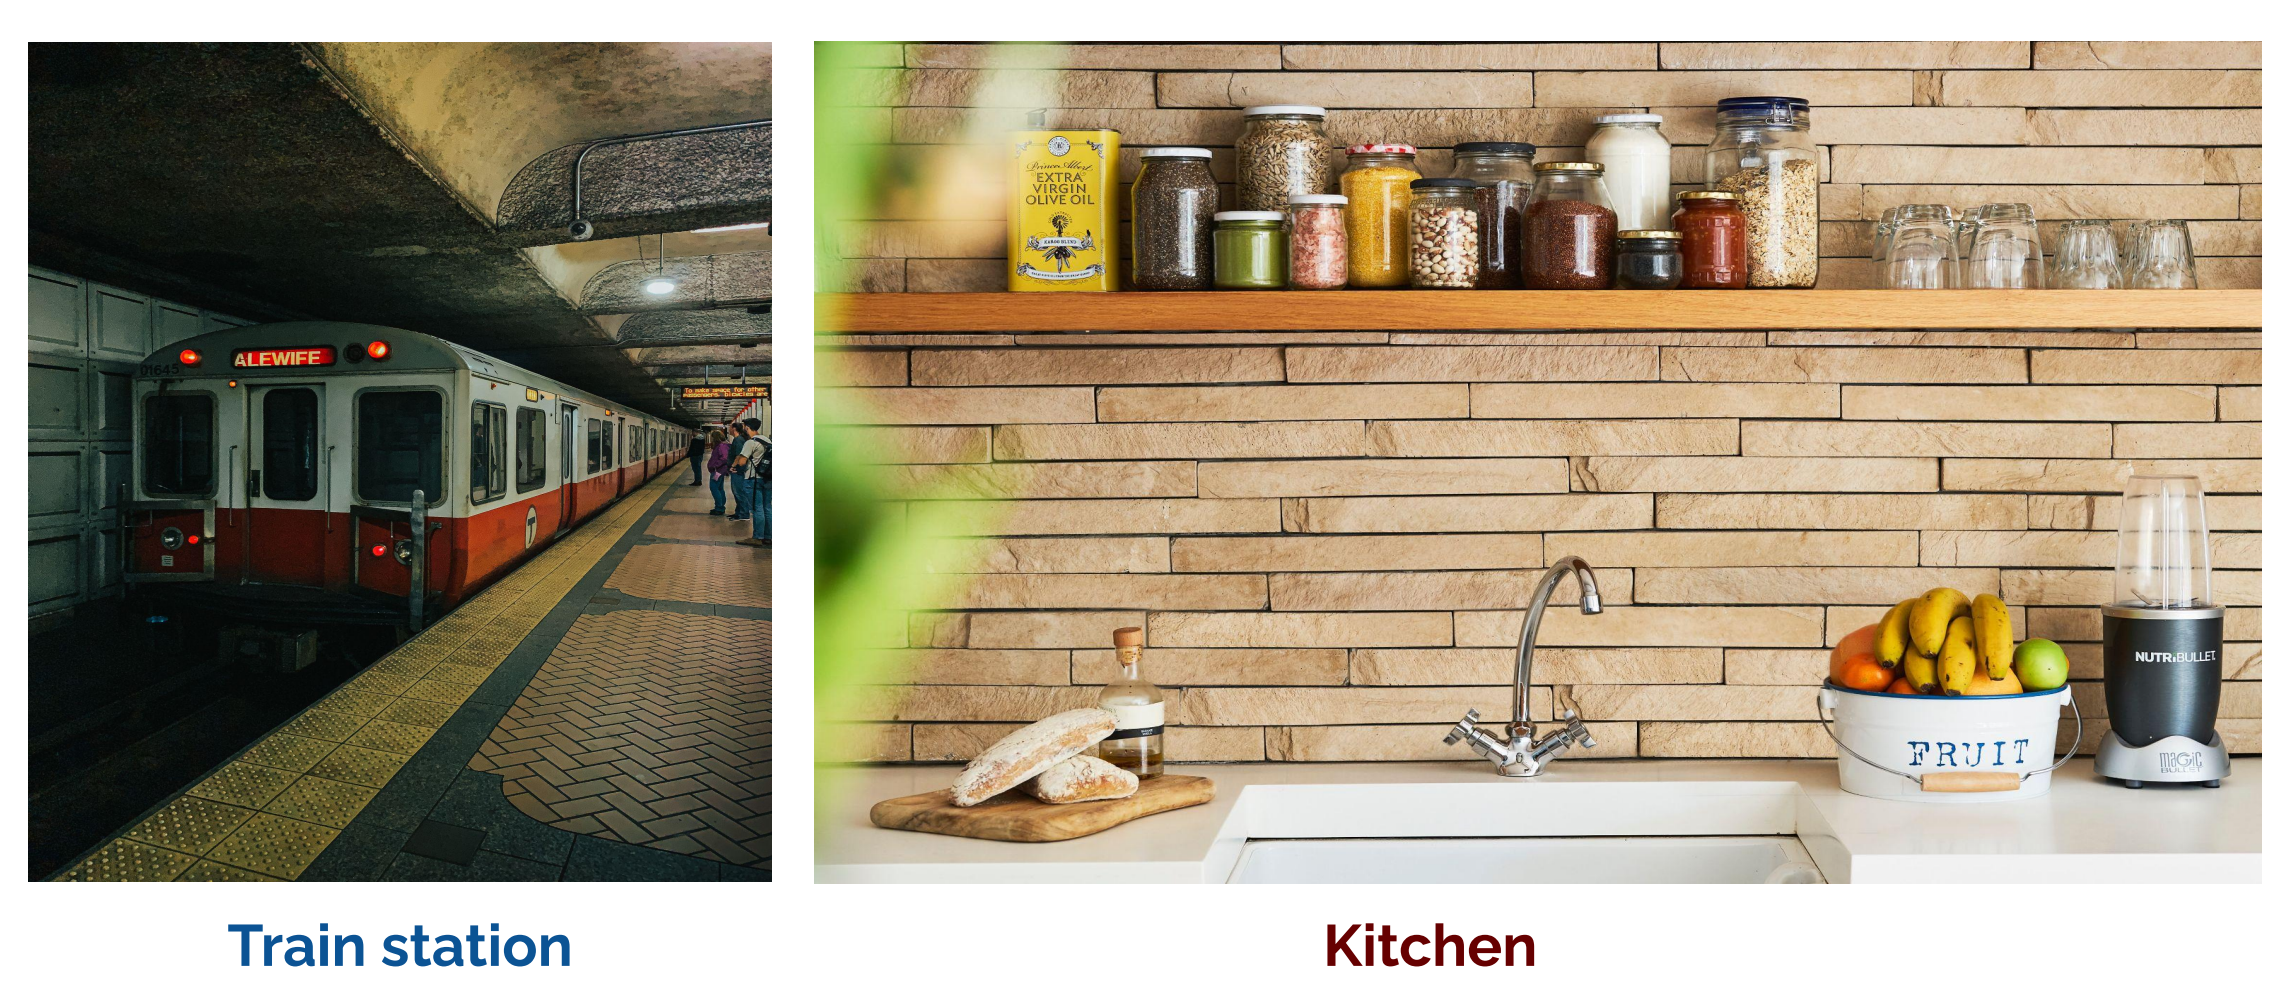
\includegraphics[width=0.6\linewidth]{figures/train_station_kitchen.png}
     \caption{Difference between visual scenes - train station and kitchen in terms of object placements.}
     \label{station_kitchen}
\end{figure}
% Use reference: \textit{Structure Inference Net: Object Detection Using Scene-Level Context and Instance-Level Relationships} here.
\section{Movies vs Natural scenes}
Visual scene recognition, in the case of static images, is primarily driven by natural scenes due to large-scale datasets like SUN397 \cite{Xiao2010SUNDL} and Places-2\cite{zhou2017places}. However, there are certain inherent challenges in visual scene recognition for movies that need to be addressed, as shown in Fig \ref{Intro figure}.
\begin{figure}[!h]
 \centering
  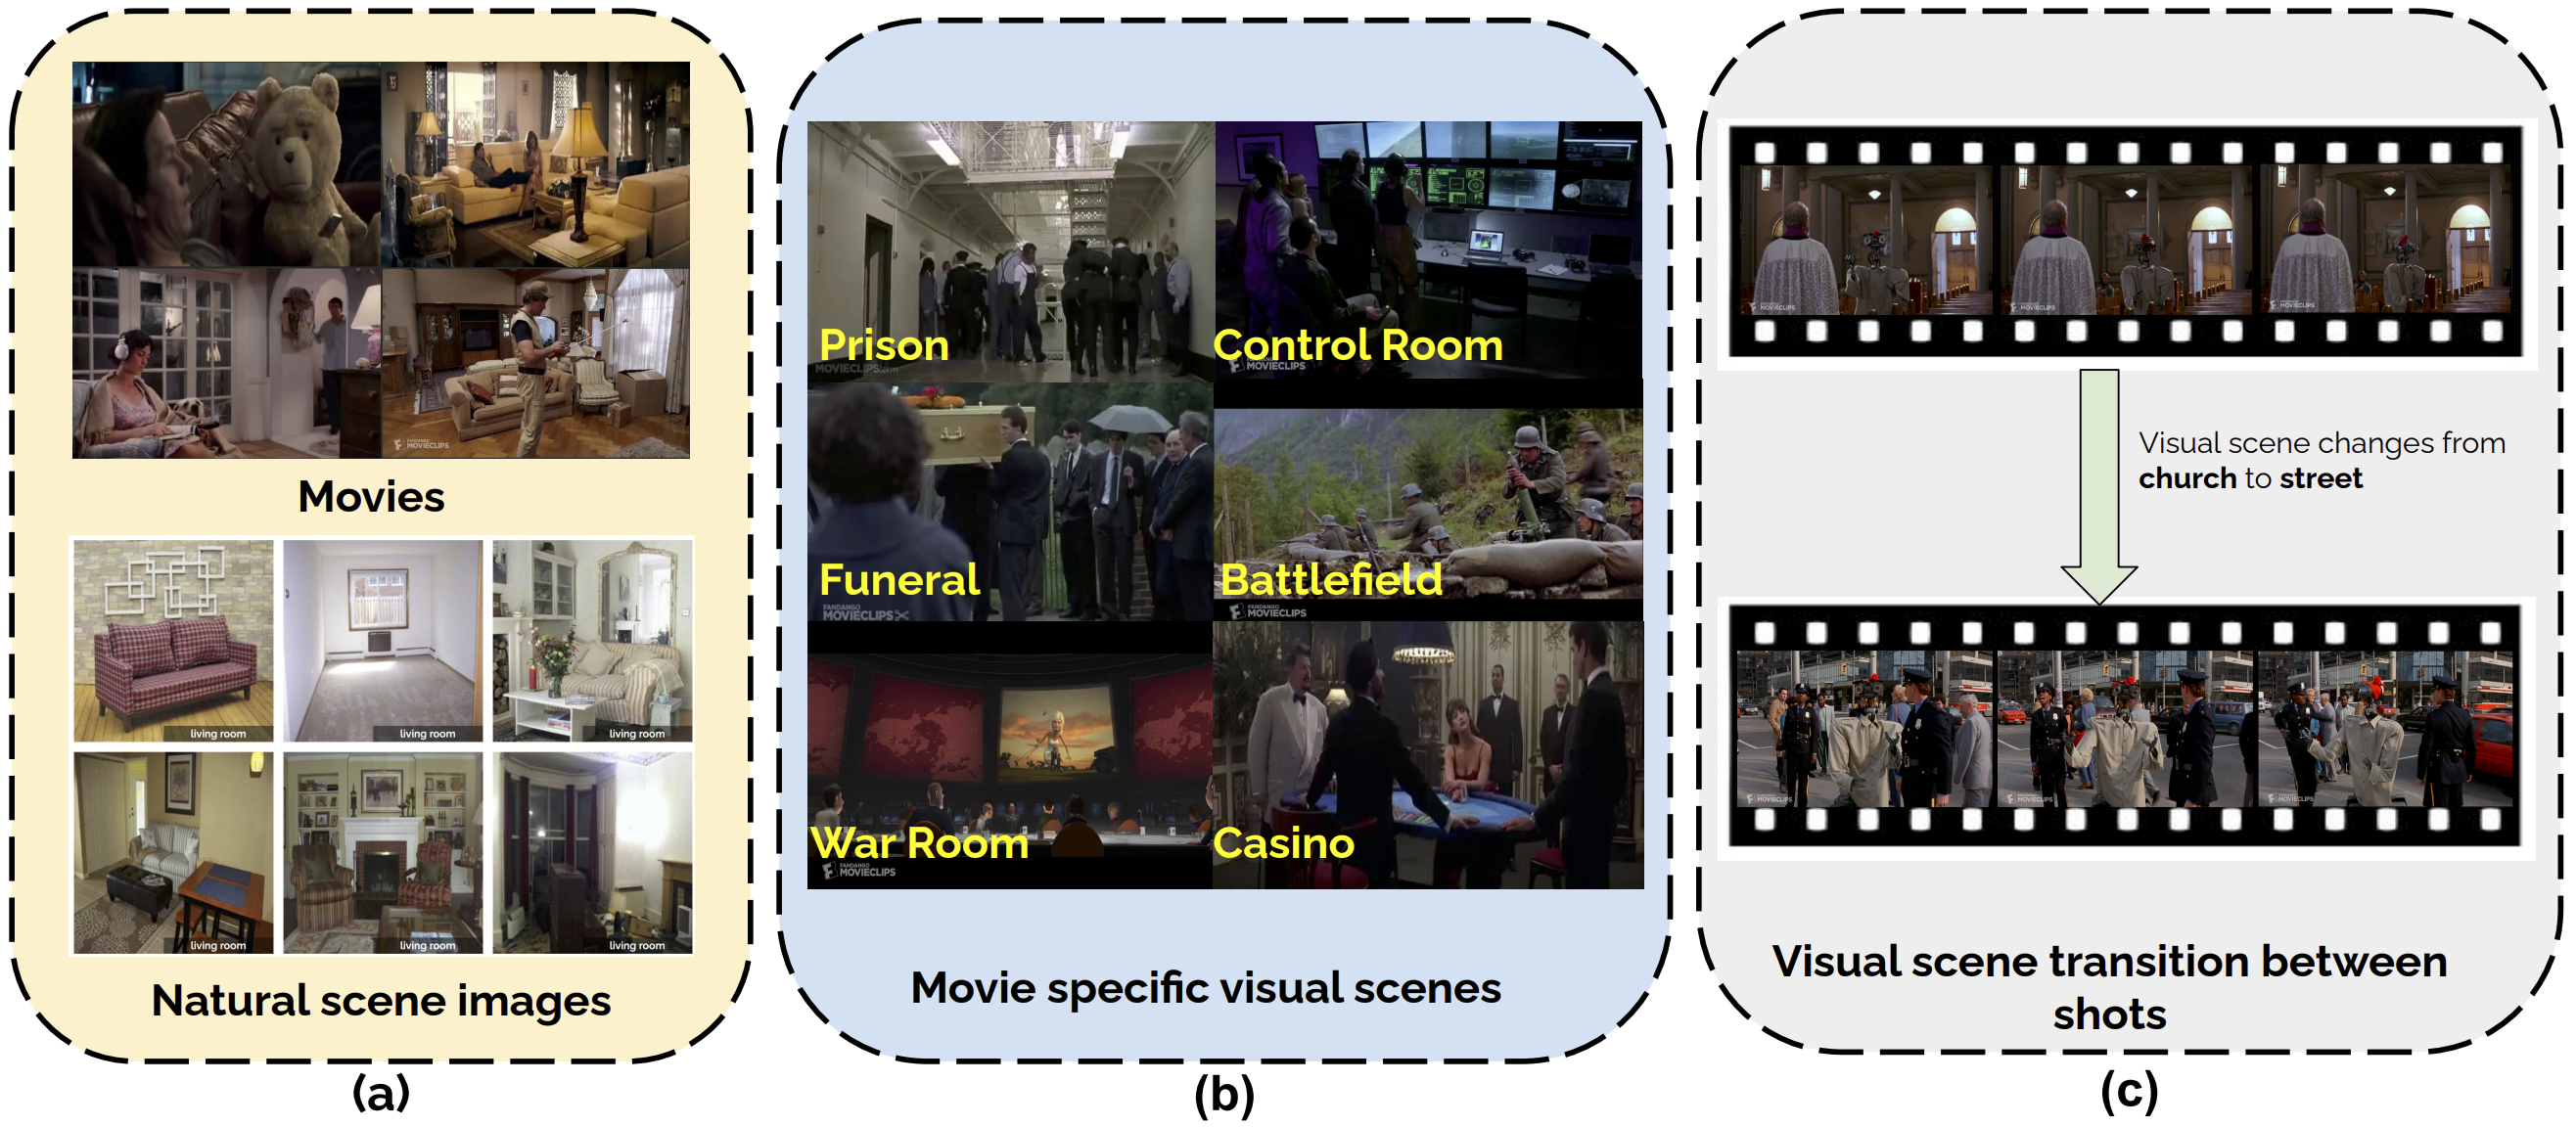
\includegraphics[width=0.8\linewidth]{figures/Introduction_Figure.png}
  \caption{Overview diagram highlighting the challenges associated with visual scene recognition in movies (a) Domain mismatch between Natural scene images,(Source: \url{http://places2.csail.mit.edu/explore.html}) vs frames from Movies for \textbf{living room} (b) Movie centric visual scene classes like prison, control room etc that are absent from existing taxonomies (c) Change in visual scene between shots in the same movie clip.}
  \label{Intro figure}
\end{figure}
\textbf{\underline{Domain mismatch - scene images vs. movie frames:}} Visual scenes depicted in movies are distinct compared to natural scenes due to increased focus on actors, multiple activities, and viewpoint variations like extreme closeup, wide-angle shots etc. An example is shown in Fig.~\ref{Intro figure} (a) for images from Places2 dataset \cite{zhou2017places} and movie frames from Condensed Movies dataset \cite{bain2020condensed}.\\
\textbf{\underline{Lack of completeness in scene taxonomy:}} Movies depict both real-life and fictional scenarios that span a wide variety of visual scenes. As shown in Fig.~\ref{Intro figure}(b), certain movie-centric visual scene classes like \textit{battlefield}, \textit{control room}, \textit{prison}, \textit{war room}, \textit{funeral}, \textit{casino} are absent from existing public scene taxonomies associated with natural scene image and video datasets.\\
\textbf{\underline{Lack of shot-specific visual scene annotations:}} Existing datasets like Condensed Movies \cite{bain2020condensed} and VidSitu \cite{Sadhu_2021_CVPR} provide a {\em single} visual scene label for the entire movie clip (around 2 minutes long), obtained through descriptions provided as part of YouTube channel Fandango Movie clips \footnote{https://www.youtube.com/channel/UC3gNmTGu-TTbFPpfSs5kNkg}. In Fig.~\ref{Intro figure} (c), the provided description: \textit{Johnny Five (Tim Blaney) searches for his humanity in the \textbf{streets} of New York.} mentions only the visual scene \textbf{street}, while the initial set of events takes place inside \textbf{church}. Instead of considering a single scene label for the entire movie clip, shot-level visual scene annotation can help in tracking the scene change from \textbf{church} to \textbf{street}.
\section{Contributions}
In our work, we consider shots within a given movie clip as the fundamental units for visual scene analysis since shots consist of consecutive set of frames related to the same content, whose starting and ending points are triggered by recording using a single camera \cite{SBD}. Our contributions are as follows:
Our contributions are as follows:
\begin{itemize}
\item \textbf{Language guided Movie-centric scene taxonomy:} We develop a movie-centric scene taxonomy by leveraging scene headers (sluglines) from movie scripts (language-based sources) and existing video datasets with scene labels like HVU\cite{diba_large_2020}. 
\item \textbf{Automatic shot tagging:} We utilize our generated scene taxonomy to automatically tag around 1.12M shots from 32K movie clips using a pretrained vision-language model called CLIP \cite{CLIP} based on a frame-wise aggregation scheme.  
\item \textbf{Multi-label scene classification:} We develop multi-label scene classification baselines using the shot-level tagged dataset called MovieCLIP and evaluate them on an independent shot-level dataset curated by human experts. 
\item \textbf{Downstream tasks:} We further extract feature representations from the baseline models pretrained on MovieCLIP and explore their applicability in diverse downstream tasks of multi-label scene and movie genre classification from web videos \cite{diba_large_2020} and trailers \cite{2019Moviescope}, respectively. 
\end{itemize}
\section{Related work}
\textbf{Image datasets for visual scene recognition:}
Image datasets for scene classification like MIT Indoor67 \cite{IndoorScenes} relied on categorizing a finite set of (67) indoor scene classes. A broad categorization into indoor, outdoor (natural) and outdoor (man-made) groups for 130K images across 397 subcategories was introduced by the SUN dataset \cite{xiao_sun_2016}. For large-scale scene recognition, the Places dataset \cite{zhou2017places} was developed with 434 scene labels spanning 10 million images. The scene taxonomy considered in the Places dataset was derived from the SUN dataset, followed by the careful merging of similar pairs. It should be noted that the curation of large-scale visual scene datasets like Places relied on crowd-sourced manual annotations over multiple rounds.\\
\textbf{Video datasets for visual scene recognition:} While there has been considerable progress in terms of action recognition capabilities from videos due to the introduction of large-scale datasets like Kinetics \cite{kinetics400}, ActivityNet \cite{caba2015activitynet}, AVA \cite{gu2018ava}, Something-Something \cite{Something-SomethingV2}, only few large scale datasets like HVU \cite{diba_large_2020} and Scenes, Objects and Actions (SOA) \cite{SOA} have focused on scene categorization with actions and associated objects. SOA was introduced as a multi-task multi-label dataset of social-media videos across 49 scenes with objects and actions but the taxonomy curation involves free-form tagging by human annotators followed by automatic cleanup. 
HVU \cite{diba_large_2020}, a recently released public dataset of web videos with 248 scene labels, relied on initial tag generation based on cloud APIs followed by human verification.\\
\textbf{Movie-centric visual scene recognition:} In the domain of scene recognition from movies, Hollywood scenes \cite{marszalek09} was first introduced with 10 scene classes extracted from headers in movie scripts across 3669 movie clips. A socially grounded approach was explored in Moviegraphs \cite{moviegraphs} with emphasis on the underlying interactions (relationships/situations) along with spatio-temporal localizations and associated visual scenes (59 classes).
For holistic movie understanding tasks, the Movienet dataset\cite{huang2020movienet} was introduced with the largest movie-centric scene taxonomy consisting of 90 place (visual scene) tags with segment-wise human annotations of entire movies. Instead of entire movie data, short movie clips sourced from YouTube channel of Fandango Movie clips were used for text-video retrieval in Condensed movies dataset \cite{bain2020condensed}, visual semantic role labeling \cite{Sadhu_2021_CVPR} and pretraining object-centric transformers \cite{transformers} for long-term video understanding in LVU dataset \cite{lvu2021}. While there is no explicit visual scene labeling, the raw descriptions available on Youtube with the movie clips have mentions of certain visual scene classes.
\\
MovieCLIP, our curated dataset for visual scene context recognition, is built on top of movie clips available as a part of Condensed Movies dataset \cite{bain2020condensed}. A comparative overview of MovieCLIP and other image and video datasets with visual scene labels is shown in Table~\ref{Overview}. In comparison with previous video-centric works, our taxonomy generation relies on domain-centric data sources like movie scripts and auxiliary world knowledge from web-video-based sources like HVU with minimal human-in-the-loop supervision for taxonomy refinement.
\begin{table*}[h!]
\centering
\resizebox{0.8\textwidth}{!}{
\begin{tabular}{|c|c|c|c|c|c|c|}
\hline
\textbf{Dataset} & \textbf{Domain} & \textbf{\#classes} & \textbf{\#samples} & \textbf{Annotation} & \textbf{Unit} & \textbf{AV} \\ \hline
Scene 15 \cite{BayesianFeiFeiLi}   & Natural & 15  & $\sim$6k   & Manual & Image  & \cmark     \\ \hline
MITIndoor67  \cite{IndoorScenes} & Natural     & 67   & 15620   & Manual  & Image &\cmark    \\ \hline
SUN397  \cite{xiao_sun_2016}   & Natural    & 397   & 130,519  & Manual  & Image &\cmark    \\ \hline
Places  \cite{zhou2017places}    & Natural   & 434   & 10m  & Manual  & Image & \cmark     \\ \hline
Hollywood Scenes \cite{marszalek09}   &  Movies    & 10    & 3669   & Automatic  & Video clip (36.1s)  & \cmark  \\ \hline
Moviegraphs  \cite{moviegraphs}    & Movies   & 59     & 7637   & Manual  & Video clip (44.28 s)  & \xmark    \\ \hline
SOA \cite{SOA} &  Web-Videos   & 49   & 562K   & Semi-automatic  & Video clip (10 s)  &   \xmark      \\ \hline
Movienet  \cite{huang2020movienet}  & Movies   & 90    & 42K  & Manual  & Scene segment (2 min)  & \xmark           \\ \hline
HVU    \cite{diba_large_2020}    & Web-Videos    & 248    & 251k  & Semi-automatic &  Video clip (10 s) & \cmark    \\ \hline
Condensed Movies \cite{bain2020condensed}   & Movies    & NA    & 33k   & Automatic  & Video clip ( 2 min) & \cmark    \\ \hline
VidSitu  \cite{Sadhu_2021_CVPR}    & Movies  & $\sim$50    & 14k   & Manual  & Video  clip (10 s) & \cmark     \\ \hline
LVU  \cite{lvu2021}    & Movies    & 6    & 723   & Automatic &  Video clip ($1 \sim 3$ min) & \cmark       \\ \hline
\textbf{MovieCLIP}  & \textbf{Movies}  & \textbf{179}  & \textbf{1.12m}& \textbf{Automatic} & \textbf{Shot (3.54s) }  & \textbf{\cmark }    \\ \hline
\end{tabular}
}
\vspace{5mm}
\caption{Comparison of MovieCLIP with other available image and video datasets with visual scene classes.  \textbf{Natural}: Images of natural scenes.\textbf{Web-Videos}: videos obtained from internet sources like YouTube. \textbf{AV}: whether publicly available or not. Avg or duration span of video data sources are provided with the respective units. \textbf{NA}: Number of scene classes explicitly not mentioned with the dataset.}
\label{Overview}
\end{table*}
\\
\textbf{Knowledge transfer from pretrained multimodal models:}
Vision language(V-L) based pretraining methods involve learning transferable visual representations based on various pretext tasks associated with image and text pairs. Examples of pretext tasks in V-L domain include prediction of masked words in captions based on visual cues in ICMLM \cite{sariyildiz2020icmlm}, pretraining image encoders based on bicaptioning objective in VirTex \cite{desai2021virtex} and contrastive alignment of image-caption pairs in CLIP \cite{CLIP}. Leveraging features from CLIP's visual and text encoders have improved existing vision-language tasks \cite{Shen2021HowMC} and enabled open-vocabulary object detection \cite{Gu2021OpenvocabularyOD}, and language-driven semantic segmentation \cite{Li2022LanguagedrivenSS}. In our work, we use the pretrained visual and text encoders of CLIP and utilize it as a noisy annotator by tagging movie shots based on our curated visual scene taxonomy.

\section{Language driven taxonomy curation}

Based on domain-specific challenges mentioned in Fig \ref{Intro figure}, we can see the need for a taxonomy curation phase for visual scenes in movies. In this section, we outline the process involved in curating a visual scene taxonomy based on the domain information present in movie scripts and the pre-existing scene information present in auxiliary video datasets.

\subsection{Sources of visual scene information}
Movie scripts have been used as external sources for describing and annotating videos through script and subtitle alignment methods in \cite{10.1007/978-3-540-88693-8_12}, \cite{Everingham2006HelloMN}, \cite{Laptevactionscvpr}, \cite{Rohrbach2015ADF}. Movie scripts contain \textit{sluglines} that provide information about visual scenes, time of the day, and whether the action takes place in indoor or outdoor settings.

\begin{figure}[!h]
 \centering
  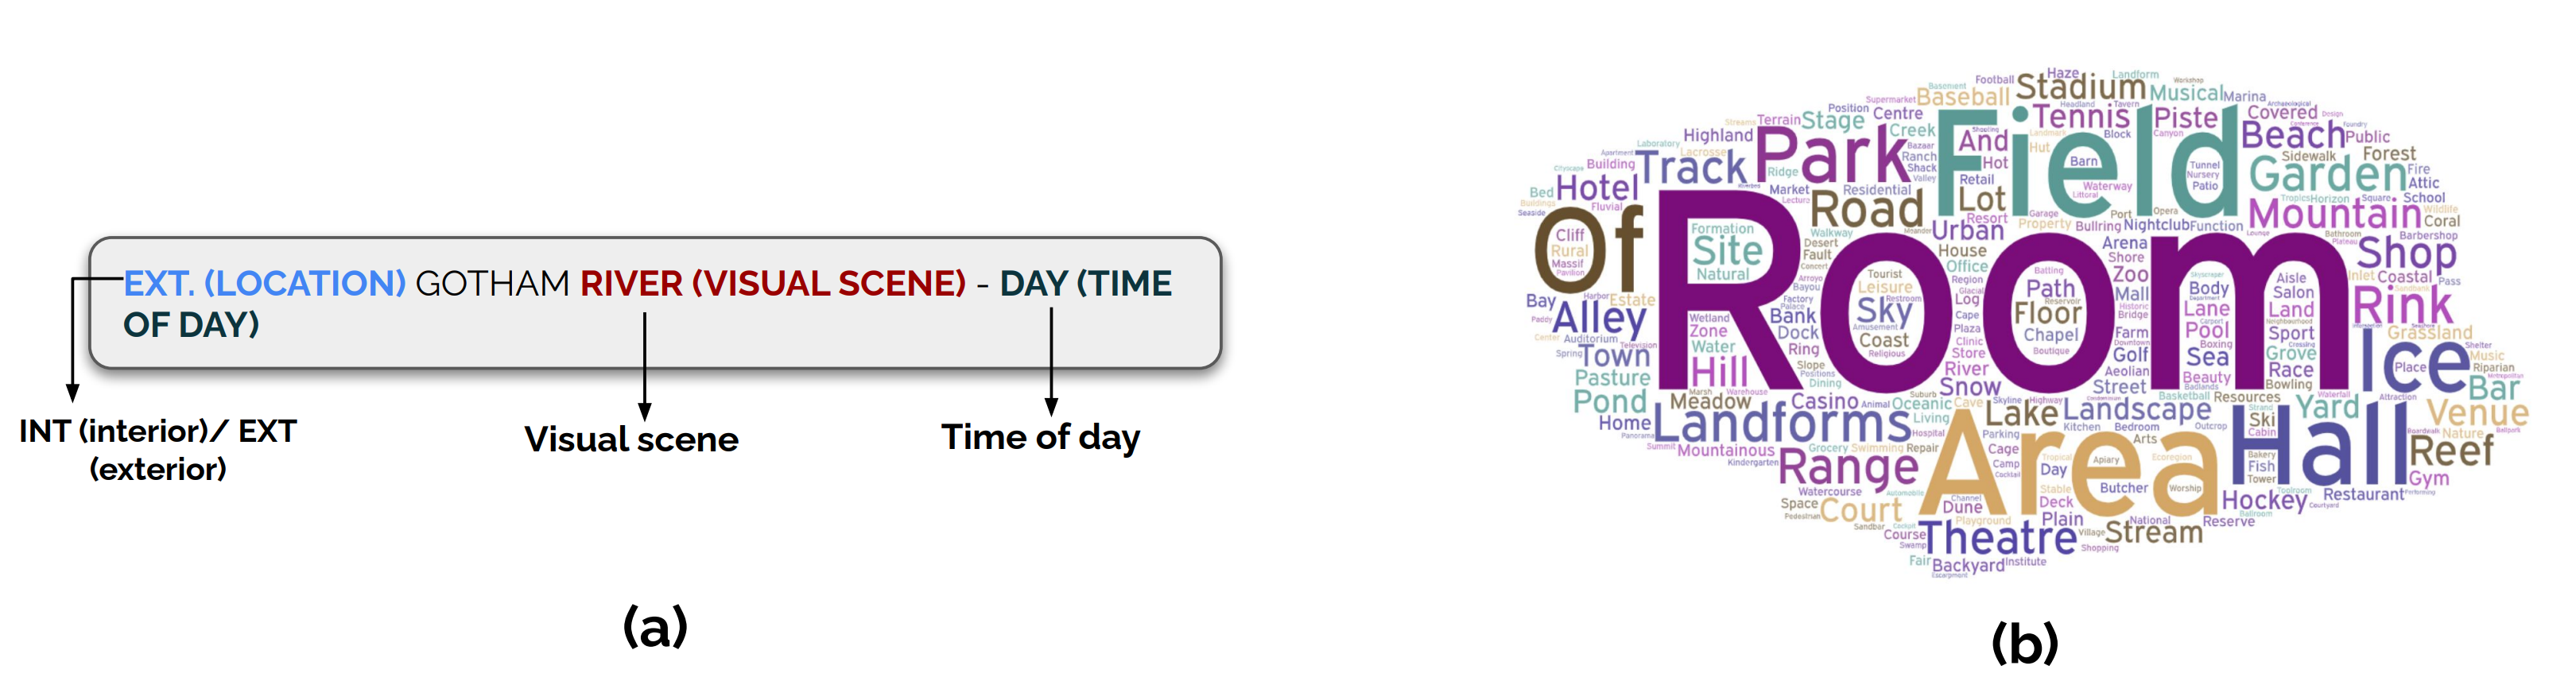
\includegraphics[width=\linewidth]{figures/sources_of_information_visual_scene_taxonomy.png}
  \caption{Sources of visual scene information: (a) Sample slugline from a movie script that contains visual scene, time of day, and location (b) Word cloud showing the distribution of visual scene labels in HVU \cite{diba_large_2020} dataset.}
  \label{sources of information}
\end{figure}

We parse 156k sluglines from an in-house set of 1434 movie scripts. For each slugline, we automatically extract entities after the ``\textbf{EXT.}''(exterior) or ``\textbf{INT.}''(interior) tags like \textit{Hospital room}, \textit{River}, \textit{War room} etc.
Using this procedure, we extract 173 unique visual scene labels. Our taxonomy generation process is motivated by visual scenes in movies with sluglines from scripts as seed sources along with auxiliary sources.
Since the set of labels from movie scripts is not exhaustive, we also consider auxiliary sources, especially web video datasets with visual scene labels like HVU \cite{diba_large_2020}. We consider HVU as source of additional labels since the taxonomy (248 visual scene classes) is semi-automatically curated for short-trimmed videos, having similar nature to movie shots. We don’t consider Places2 \cite{zhou2017places} dataset since the taxonomy is primarily curated for natural
scenes, which are distinct from movie-centric visual scenes. Sample slugline from a movie script and a word cloud showing the distribution of visual scene labels is shown in Fig \ref{sources of information}.

\subsection{Visual scene taxonomy curation}
In order to develop a comprehensive taxonomy of visual scenes in movies, we develop an automatic way of merging taxonomies from movie sluglines and the auxiliary dataset i.e., HVU with minimal human-in-the-loop for post-processing. The broad steps involved in the taxonomy generation are listed as below:
\par
\textbf{Label space preprocessing:} For simplicity, we consider the set of unique labels from movie sluglines (MS) to be denoted as $L_{MS}$ and its cardinality as $N_{MS}$. Similarly we denote $N_{HVU}$ to be the cardinality of the set $L_{HVU}$, i.e., the set of unique labels from the HVU dataset. For our case, we have $N_{MS}=173$ and $N_{HVU}=248$. We extract the intersecting set of labels between $L_{MS}$ and $L_{HVU}$, denoted by the set $L_{com}$ . The number of common labels between HVU and movie slugline based taxonomy is $N_{com}=68$. We remove the common set of labels $L_{com}$ from both the label spaces of movie sluglines and HVU. This gives us a non-intersecting set of labels in movie sluglines and HVU denoted by $L_{MS} \setminus L_{Com}$  and $L_{HVU} \setminus L_{Com}$ respectively.  We combine the sets of labels i.e. $L_{MS} \setminus L_{Com}$ and $L_{HVU} \setminus L_{Com}$ to obtain a larger set of labels called $L_{NC}$, where NC refers to not common. 
\begin{equation}
    L_{NC}=(L_{MS} \setminus L_{Com}) \cup (L_{HVU} \setminus L_{Com})
\end{equation}
\par 
\textbf{Merging with common label space:}
In this step, we find labels in $L_{NC}$ that are semantically close to the labels in $L_{com}$. We extract dense 384D label representations using the MiniLM-L6-v2 sentence transformers model \cite{reimers-2019-sentence-bert} for labels in $L_{NC}$ and $L_{com}$. For each label in $L_{NC}$ we compute cosine similarities with set of labels in $L_{com}$ based on label representations. We merge those labels from $L_{NC}$ with the similar labels in $L_{com}$, whose top-1 cosine similarity values are greater than 0.6. We update the set of labels $L_{NC}$ to $L_{N}$ by removing the merged labels.
Examples of such merging with respective cosine similarities and sources are as follows:

\begin{itemize}
    \item $\textbf{dune} \{L_{NC}\} \rightarrow{} \textbf{desert} \{L_{com}\} (0.66)$ 
    \item $\textbf{tennis} \ camp \{L_{NC}\} \rightarrow{} \textbf{tennis \ court} \{L_{com}\}  (0.62)$
    \item $\textbf{restroom} \{L_{NC}\} \rightarrow{} \textbf{bathroom} \{L_{com}\} (0.80)$
    \item $\textbf{rural \ area} \{L_{NC}\} \rightarrow{} \textbf{village} \{L_{com}\} (0.64)$
    \item $\textbf{boardwalk} \{L_{NC}\} \rightarrow{} \textbf{walkway} \{L_{com}\} (0.67)$
    \item $\textbf{television \ room} \{L_{NC}\} \rightarrow{} \textbf{living \ room} \{L_{com}\} (0.67)$
    \item $\textbf{glacial \ lake} \{L_{NC}\} \rightarrow{} \textbf{lake} \{L_{com}\} (0.73)$
\end{itemize}

\begin{figure}[h!]
\centering
%\subfloat[]{%
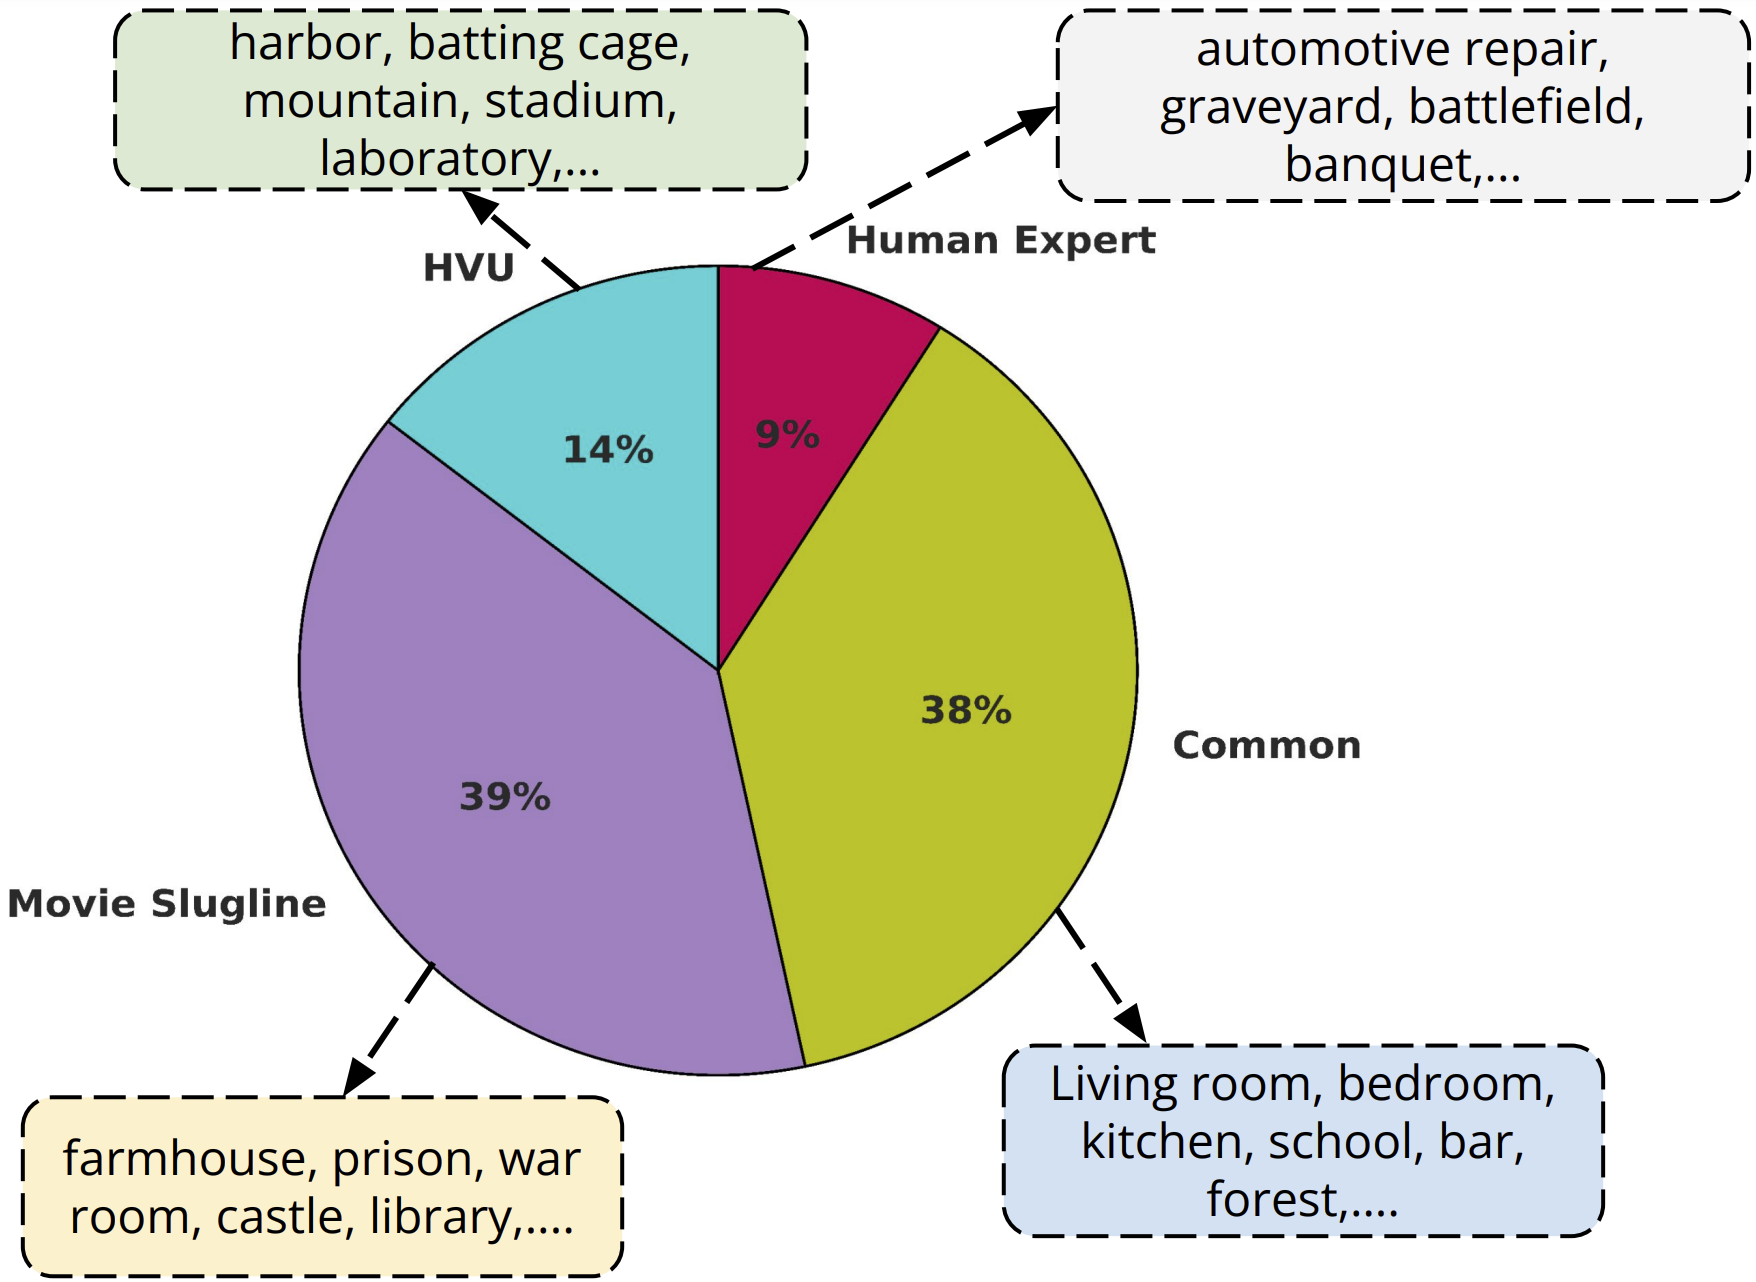
\includegraphics[width=0.6\columnwidth]{figures/share_of_labels.png}%
\caption{
The share of different sources (\textbf{HVU}, \textbf{Movie Sluglines}, \textbf{Common labels and Human expert}) in curating the label taxonomy. Example labels from different sources are shown in boxes with the pie chart.
}
\label{label distribution}
\end{figure}
\textbf{Human-in-the-loop taxonomy refinement:} 
A human expert inspects the labels in $L_{N}$ and removes both generic scene labels such as \textit{body of water}, \textit{coastal and oceanic landforms}, \textit{horizon}, \textit{landscape}, \textit{underground} as well as highly specific scenes such as \textit{coral reef}, \textit{white house}, \textit{piste}, \textit{badlands} etc. We use label representations from the previous step to exploit semantic similarity between the labels remaining in $L_{N}$.
For each relevant label in $L_{N}$, a threshold of 0.7 on top-1 similarity score is used to filter out similar labels. While comparing two similar labels, the human expert relies on wiki definitions to merge the more specific label into the generic one. For example, by definition \textit{bazaar} is a special form of market selling local items (as per wiki) and therefore merged with the \textit{market}. Other examples include:
\begin{itemize}
    \item $\{stream, river bed, creek, river\} \rightarrow{} river$ 
    \item $\{hill, mountain, mountain \ pass, mountain \ range\} \\ \rightarrow{} mountain$
    \item $\{road, road \ highway, lane \} \rightarrow{} road$
    \item $\{port, marina \ dock, harbor \} \rightarrow{} harbor$
\end{itemize}
This results in a set of labels called $L_{merge}$ from $L_{N}$. Further, The human expert is exposed to randomly sampled 1000 shots from movie clips in Condensed Movies \cite{bain2020condensed} and reviews the current set of labels in the set $L_{merge} \cup L_{com}$. Based on the video content, a set of scene labels ($L_{human}$) that are missing from the current set is added by human expert. Thus the final set of 179 visual scene labels is obtained as follows:
\begin{equation}
     L_{final}=L_{com}\cup L_{merge} \cup L_{human}
\end{equation}
\textbf{Label source distribution:} As shown in Fig. \ref{label distribution}, the largest share is from movie sluglines (39\%).Only 9\% of the total labels is provided through feedback from human expert. Instead of manually binning classes into broad categories like indoor, outdoor or man-made, we discover groupings among classes through Affinity propagation clustering \cite{brendanfrey}  (based on label representations from sentence transformers). Certain clusters of visual scene labels are listed below, where all the sport locations, water bodies and performing arts locations are grouped together.
\begin{itemize}
    \item \textbf{sport locations:} Basketball court, Race track, Tennis court, Batting cage, Golf course
    \item \textbf{water bodies:} River, Pool, Waterfall, Hot spring, Pond, Swamp, Lake
    \item \textbf{performing arts locations:} Stage, Conference Room, Theater, Auditorium, Ballroom
    \item \textbf{Natural landforms:} Mountain, Desert, Valley
\end{itemize}
For visualizing certain groups of visual scene classes that are semantically close to each other, we use tSNE \cite{tSNE} to project the 384 D label embeddings obtained through MiniLM-L6-v2 sentence transformers model \cite{reimers-2019-sentence-bert} to 2 dimensions. Examples include the visual scene classes associated with \textbf{study}, \textbf{water bodies} , \textbf{medical scene classes}, \textbf{natural landforms}, \textbf{automobile-based scene classes}, \textbf{dining-scene classes}.
\begin{figure*}[h!]
    \centering
    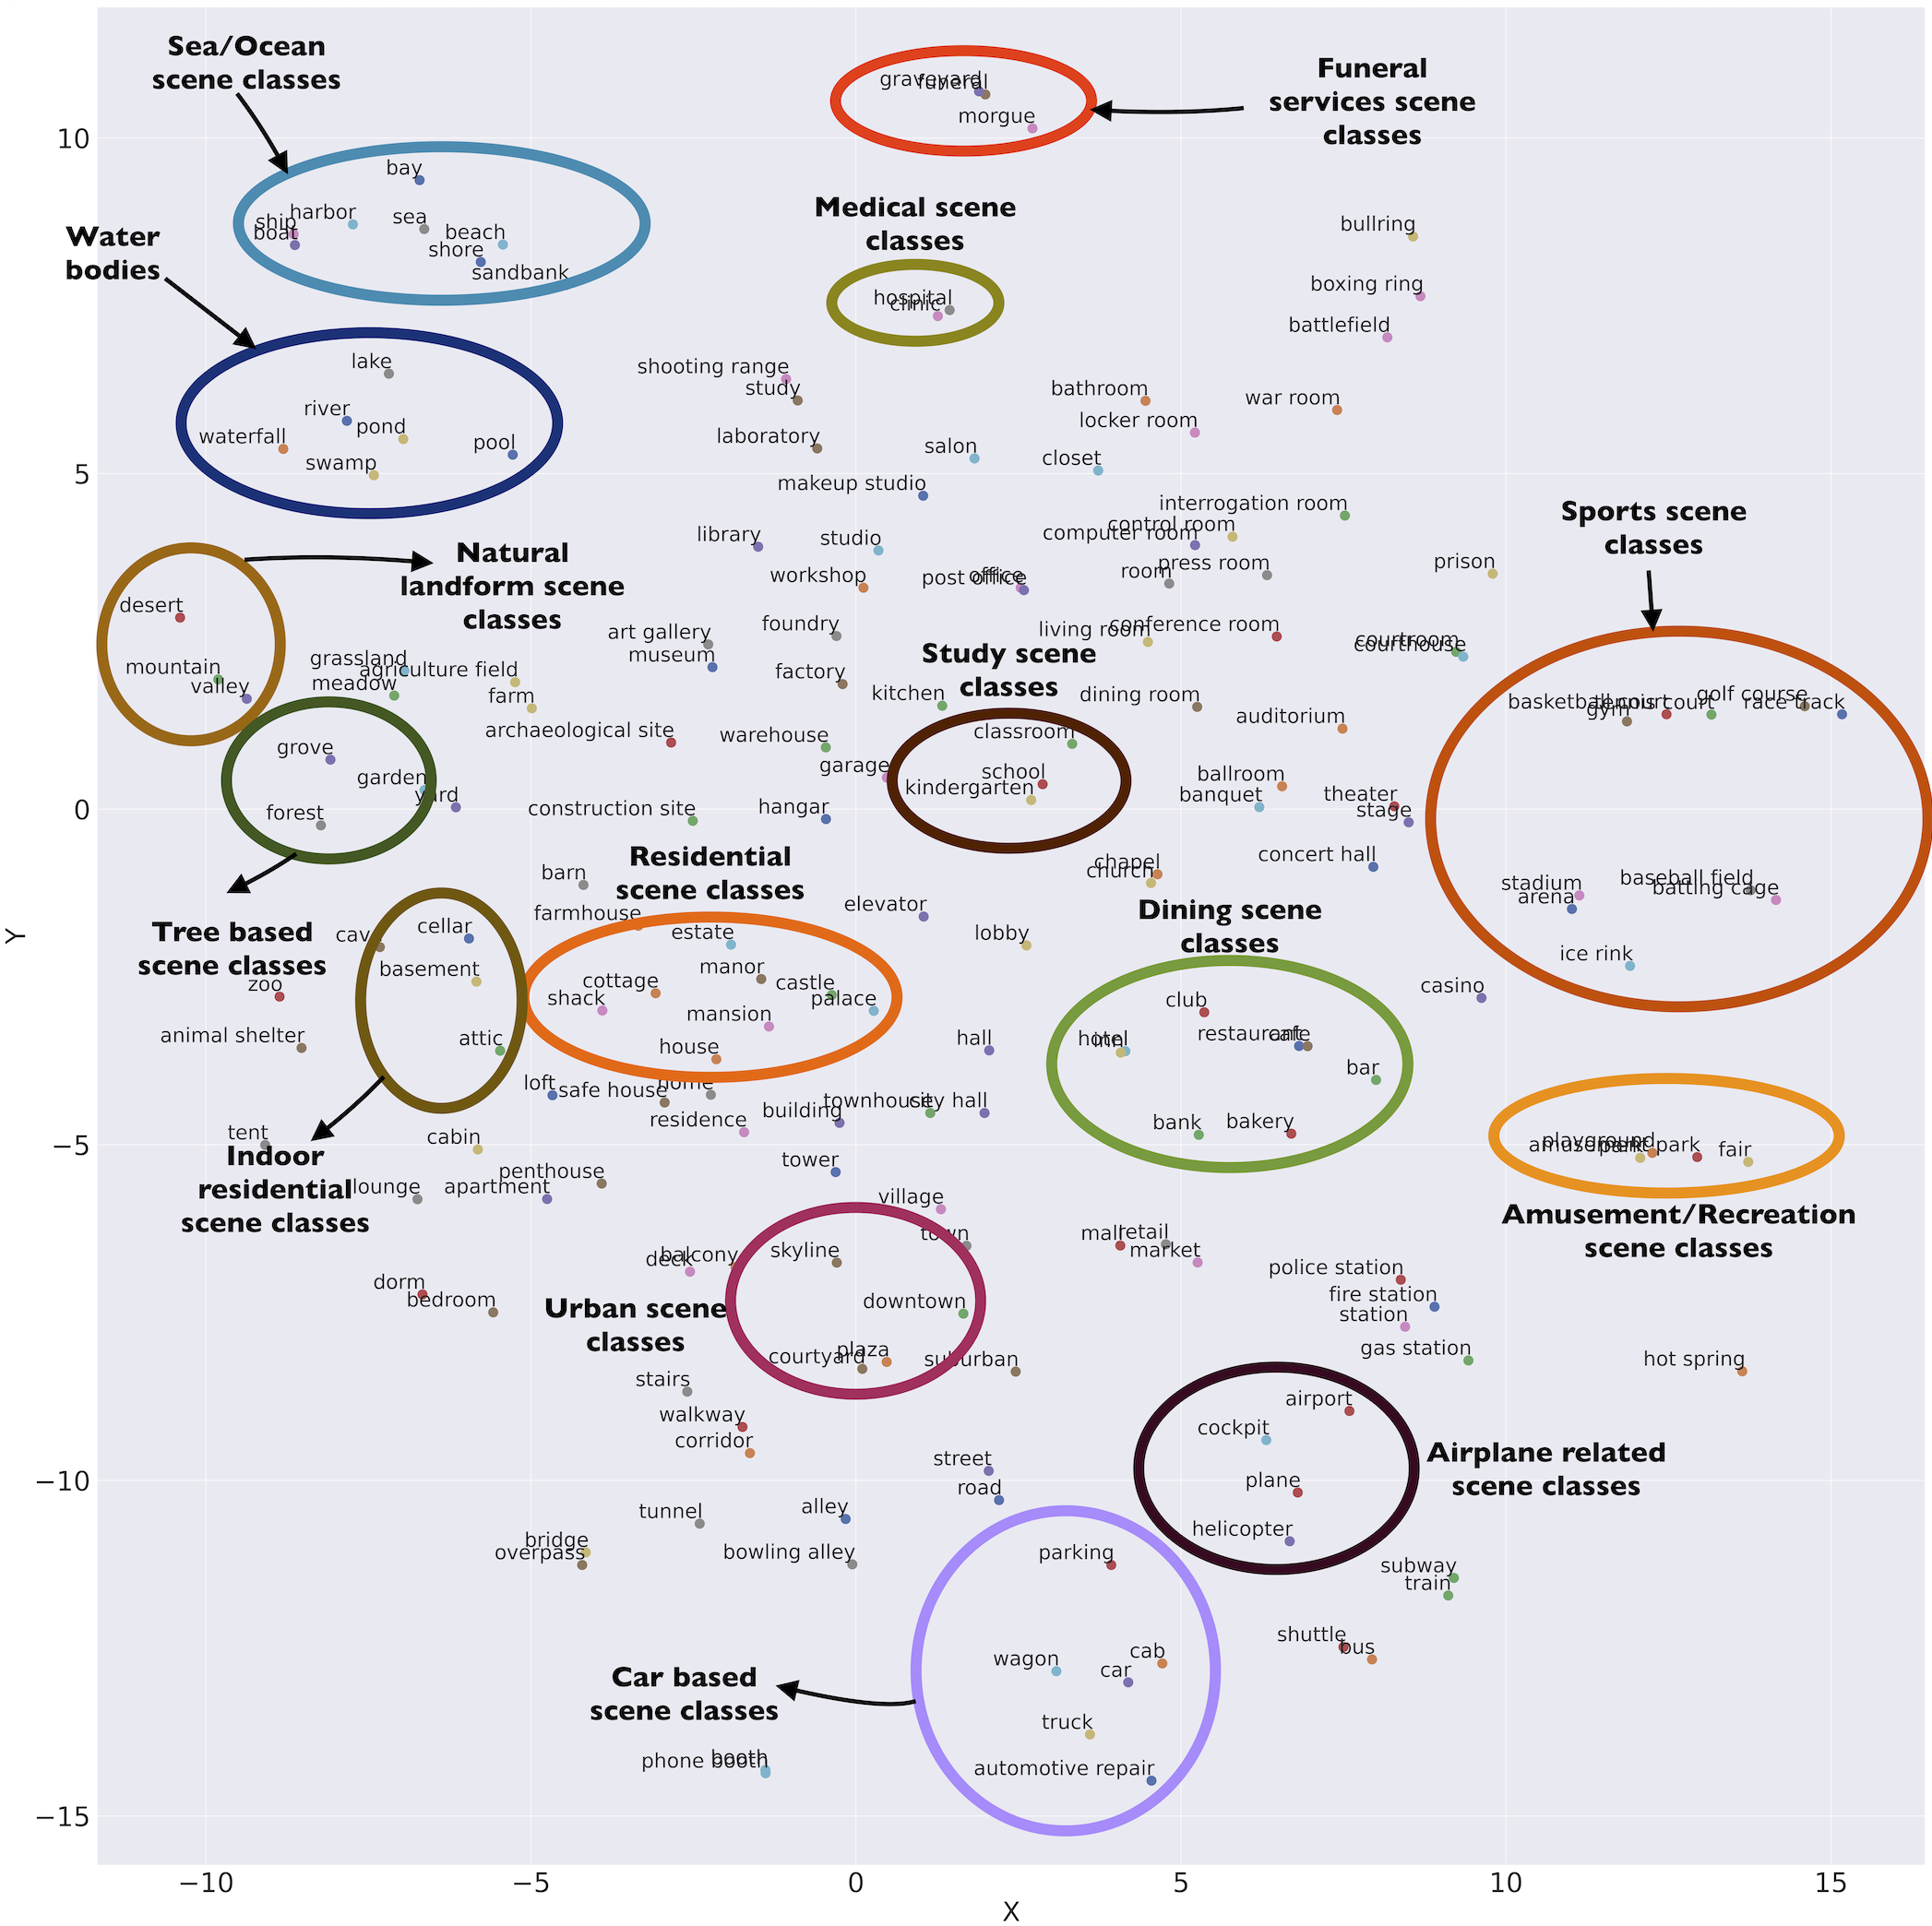
\includegraphics[width=0.9\textwidth]{figures/tsne_hvu_slugline_combined.png}
    \caption{TSNE plot of the 179 scene classes in the taxonomy. Certain representative groups of visual scene labels that are semantically close to each other are enclosed by circular/oval shapes. }
    \label{tsneplot}
\end{figure*}

\section{Role of multi-modality - Usage of vision-language models}

Since the manual tagging of Condensed Movies \cite{bain2020condensed} is not feasible due to the duration of data involved, i.e., \textbf{1106 hrs},  we ask the following question:  \textit{Can we use additional knowledge sources to provide weak guidance for the tagging task ?}. In this case, we leverage the pretrained knowledge available as part of CLIP \cite{CLIP}'s vision and language encoders to provide weak guidance for visual scene labeling. 

\begin{figure}[h!]
\centering
  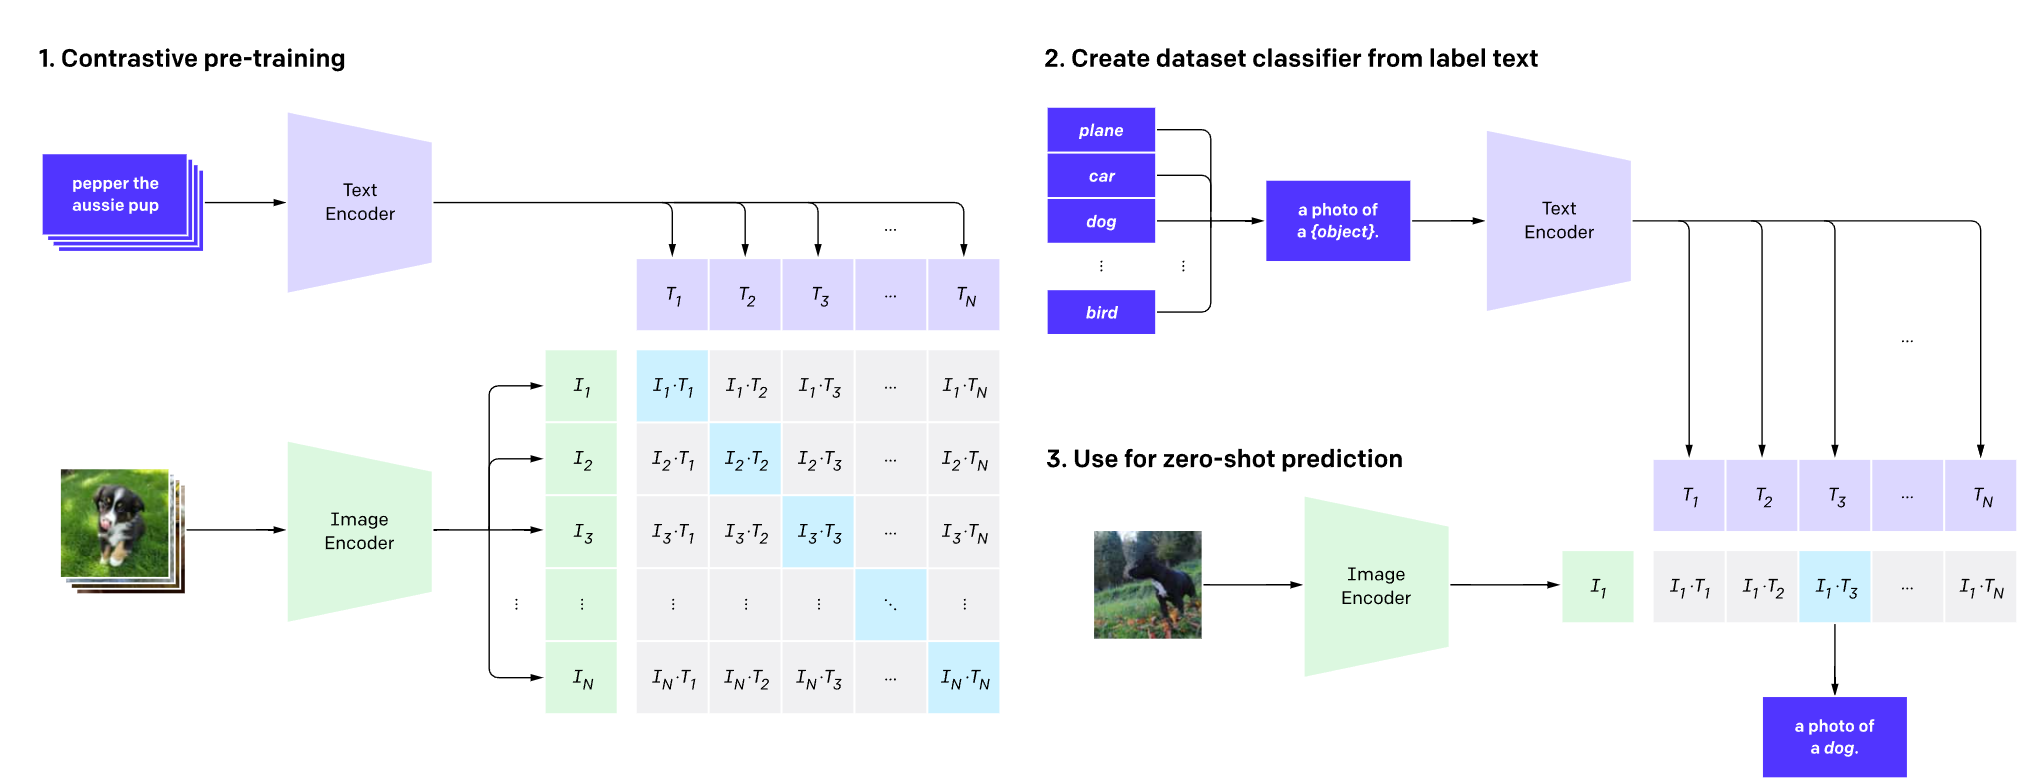
\includegraphics[width=\linewidth]{figures/CLIP_outline_diagram.png}
  \caption{1. Contrastive pretraining framework associated with CLIP. 2. Usage of CLIP's pretrained vision and text encoders for zero-shot classification. Image source: \cite{CLIP}}
  \label{CLIP outline}
\end{figure}

\subsection{CLIP: Learning Transferable Visual Models From Natural Language Supervision}
\subsection{MovieCLIP dataset}
\subsection{CLIP-based visual tagging}
\subsection{Analysis of CLIP tagging}
\subsection{Quality estimation through human verification}
\section{Experiments and Results:}
\subsection{Experimental Setup}
\subsection{Visual scene recognition - Movies}
\subsection{Downstream tasks}
\subsubsection{Visual scene recognition - web videos}
\subsubsection{Multi label genre classification - movie trailers}
\subsubsection{Impact of MovieCLIP pretraining}
\section{Ethical implications}
\section{Conclusion}
